\documentclass{llncs}
\usepackage[utf8]{inputenc}
\usepackage[russian]{babel}
\usepackage[pdftex]{graphicx}
\usepackage{comment}
\usepackage{cite}
\usepackage{cmap}
\usepackage{setspace}
\usepackage{authblk}
\usepackage{amsmath}
\usepackage{amssymb}
\usepackage{siunitx}

\graphicspath{{pic/}}
\DeclareGraphicsExtensions{.eps,.pdf,.png,.jpg}

\usepackage{tabularx}
\usepackage{multicol}
\usepackage{epstopdf}

\usepackage{subfig}
\usepackage[font={footnotesize,sl}]{caption}

% Номера страниц сверху и по центру
%\def\headfont{\small}
%\pagestyle{headcenter}
%\chapterpagestyle{empty}

\pagestyle{plain}

% Использовать полужирное начертание для векторов
\let\vec=\mathbf

% Включать подсекции в оглавление
\setcounter{tocdepth}{2}

\usepackage{indentfirst}

\usepackage{bm}
\usepackage{empheq}
\usepackage{longtable}
\usepackage{multirow}
\usepackage{multicol}
\usepackage{tikz}
\usetikzlibrary{shapes,shapes.geometric,arrows,fit,calc,positioning,automata}
\usetikzlibrary{arrows.meta}
\usetikzlibrary{shapes.multipart}
\usetikzlibrary{patterns}
\usetikzlibrary{decorations.pathreplacing}

\usepackage{extarrows}
\usepackage{rmathbr}
\usepackage{embrac}
\usepackage{todonotes}


\title{Исследование эффекта скрытых станций в сетях Wi-Fi с учетом захвата канала}
\author{
Глинский К., Куреев А.\\
\{kglinsk\}@yandex.ru, \{kureev\}@iitp.ru\\
}
\institute{ИППИ РАН}

\begin {document}
\maketitle

\begin{abstract}
В сетях стандарта 802.11 реализован алгоритм случайного доступа, требующий обеспечивать равномерное распределение ресурсов по участникам сети. При пересечении двух кадров от разных источников приемник может просигнализировать о коллизии и не принять ни один из кадров. Тем не менее, если существенно более слабый сигнал поступил раньше, то существует  возможность произвести пересинхронизацию и принять более сильный при достаточном соотношении мощностей. Данный эффект называется эффектом захвата канала. В данной работе для экспериментального изучения эффекта используется  программно-определяемое радио NI USRP 2944 RIO, на котором в рамках  исследования  был имплементирован эффект захвата канала.
\end{abstract}

\keywords{Эффект захвата канала, USRP, скрытые станции, IEEE 802.11 }

\section{Введение}
В настоящее время технология беспроводных сетей стандарта 802.11 широко распространена, и прогнозируется дальнейший рост как количества подключенных устройств, так и обьемов передаваемых по сети данных. Таким образом, актуальными становятся исследования механизмов, позволяющих повысить пропускную способность и снизить задержки в условиях плотных сетей и высоких показателей загрузки каналов сети, а также снизить влияние соседствующих и интерферирующих станций. Одним из таким механизмов является эффект захвата канала, который способен существенно повысить пропускную способность сети в некоторых сценариях использования сети. Данный эффект заключается в возможности декодировать более сильный сигнал при пересечении кадров при передаче в одном диапазоне частот.Эффект захвата канала изучен методами математического моделирования при различных предположениях о параметрах сети. Проводилось и имитационное моделирование данного эффекта. Тем не менее, проведенные  экспериментальное исследования требовали либо сложной архитектуры и методологии проведения эксперимента, либо могли проводиться на основе off-the-shelf сетевых устройств с изменением работы  только на уровне драйверов оборудования. Новизна данной статьи состоит в том, что устройство с эффектом реализовано на программно-конфигурируемом оборудовании.
\section{Эффект захвата канала в сетях 802.11}
Стандарты 802.11 определяют структуру кадра и распределение ресурсов между участниками сети. В качетсве алгоритма случайного доступа используется метод CSMA/CA, регламентирующий  доступ к каналу и механизм разрешения коллизий. В отсутстие эффекта захвата, оба пакета будут считаться недействительными. Однако, если эффект захвата канала реализован, то возможно принять более сильный кадр, если разница мощностей между ними $\Delta$W превосходит необходимое для используемой сигнально-кодовой конструкции соотношение сигнал-шум. В таком случае можно выделить два варианта.
\begin{enumerate}
\item Более мощный пакет приходит первым, успешно проходит синхронизация и прием данных, слабый же пакет теряется. Данный вариант изображен на рис\\
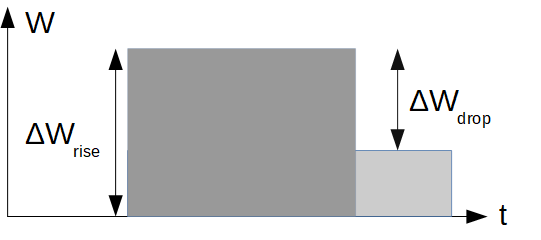
\includegraphics[scale=0.5]{capture effect init.png}
 
\item Более мощный пакет приходит вторым, и приемник уже синхронизировался на первы слабый пакет. В таком случае второй пришедший пакет приводит к потере информации из обоих пакетов в отстутствие эффекта, и приему сильного в случае пересинхронизации на него.
\\
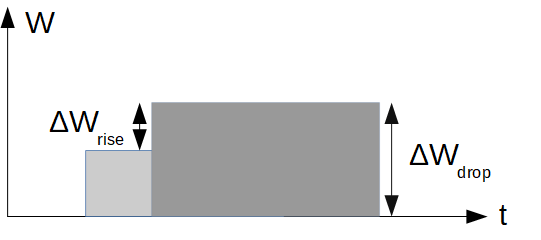
\includegraphics[scale=0.5]{capture effect scenario 1.png} 
\end{enumerate}

\section{Имплементация алгоритма в USRP}
\subsection{Аппаратная часть используемого оборудования}
Аппаратная часть используемого оборудования может быть разбита %при броске из окна
на несколько подсистем, что отображено на схеме


\subsection{Формулировка требований к алгоритму}
К алгоритму, реализованному в USRP для наблюдения эффекта захвата канала,  предьявляются следующие требования
\begin{enumerate}
\item Обладать  обратной совместимостью с оборудованием не поддерживающим данный эффект, и соответствовать основным требованиям различных редакций стандарта 802.11
\item Иметь возможность регулировать предельные параметры  сигналов, при которых  начинает происходить пересинхронизация приемника. 
\item Обеспечивать корректное начала приема более сильного сигнала вместе с освобождением всех данных слабого пакета из памяти и буферов обмена, тем самым разделяя обработку данных принятых из двух пакетов вне зависимости от сдвига по времени двух пакетов между собой.
\item Не допускать ложных срабатываний эффекта при различных сценариях 
использования устройства.
 
\end{enumerate}  В качестве
основного признака, на основании которого можно предполагать коллизию двух пакетов с различными параметрами, было выбрано изменение значение мощности входящего сигнала во время приема пакета на величину выше определенного порога. Данный признак был выбран в силу следующих предположений \begin{enumerate}
\item Мощность сигнала от одной станции слабо меняется в течении передачи одного кадра. 
\item Характеристики канала также не изменяются за время порядка одного пакета. 
\item Детектирование эффекта должно быть произведено и обработано за минимально возможное время.

\end{enumerate} 
Условие срабатывания эффекта по превышению порога мощности удовлетворяет поставленным условиям, так как согласно стандарту 802.11 дрейф мощности станции не превышает 5 db ,а вычисление мощности входного радиосигнала выполняется за 64 элементарных отсчета, каждый из которых составляет 12,5 нс.
\\\
\subsection{Алгоритм реализованного эффекта}
После обнаружения скачка входной мощности логическая защелка устанавливается в новое состояние, не допуская дальнейшие избыточные попытки пересинхронизации до прихода сигнала сброса защелки. Сигналом сброса выступает падение входной мощности на величину выше порога, сигнализирующая о завершении кадра и готовности к принятию следующих.
Логическая схема данного модуля представлена на рис. 2.
\\\
После срабатывания данного эффекта происходит переключение машины состояний, реализованной внутри FPGA USRP в состояние поиска синхронизации ( частей пакета L-STF и L-LTF). Одновременно происходит перенастройка модулей AGC (automatic gain control), вычисляющий коэффициент усиления для входного сигнала, и модуля CFO (Central frequency offset), устанавливающий величину сдвига частоты относительнно эталонной. Также на этом этапе происходит очистка памяти декодера Витерби и десериализатора в модуле побитовой обработки. %?????
\\\
Далее происходит обработка и принятие данных более сильного пакета до завершения приема и сигнала о принятии последнего сэмпла, после чего происходит сброс защелки эффекта захвата (вследствие падения мощности радиосигнала) и станция становится готова к приему следующего пакета.



\section{Экспериментальная проверка эффекта}
Для экспериментальной проверки работоспособности устаноки использовался сценарий эффекта захвата с двумя станциями-передатчиками, отправляющими пакеты с заданными разностью мощностей сигналов и сдвигом по времени (меньше длины пакета). Схема данного эксперимента приведена на рисунке ниже. 
\\\
 \begin{figure}[ht!]
\centering
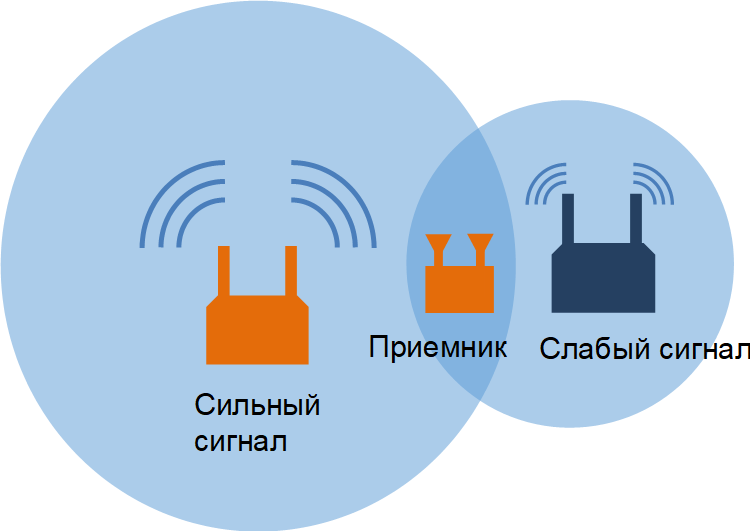
\includegraphics[width=\linewidth]{capture effect scheme.png}
\caption{Схема эксперимента \label{overflow}}
\end{figure}
\section{Заключение}
Сети стандарта 802.11 стандарта 802.11 подвержены влиянию эффекта захвата канала, способному влить на сети.
Задачей данной работы было создать установку, способную производить прием пакетов  с учетом эффекта захвата канала.
В рамках данной работы был реализован программно-аппаратный комплекс на базе USRP NI 2944 RIO для исследования эффекта захвата канала c возможностью настройки параметров  детектирования эффекта. Созданный программно-аппаратный комплекс был протестирован в сценарии со скрытыми станциями и его работоспособность была экспериментально подтверждена. 
 

%\bibliographystyle{ugost2008}
%\bibliography{biblio}

\end{document}
